\documentclass[conference]{IEEEtran}

\usepackage{amsmath,amssymb}
\usepackage{booktabs}
\usepackage{graphicx}
\usepackage{microtype}
\usepackage{url}

\title{Hierarchical Device--Edge--Cloud Task Offloading:\\
Implementation Audit and Reproducible Simulation Baselines}

\author{
\IEEEauthorblockN{Student 1 and Student 2}
\IEEEauthorblockA{INSAT, Tunis, Tunisia\\
\{student1,student2\}@example.invalid}
}

\begin{document}
\maketitle

\begin{abstract}
This paper documents an auditable implementation of hierarchical task
offloading across device, edge, and cloud tiers. The repository provides a
discrete-event SimPy backend with separate device-placement, edge-placement,
and cloud-queue decisions, shared resource queues, network serialization, and
device energy accounting. Four Double-DQN adapters are integrated at the
policy boundary, but their current formulation assigns terminal credit to
each task decision and is therefore a contextual one-step formulation rather
than a sequential multi-agent Gymnasium environment. The committed
quantitative evidence is a three-seed, ten-task synthetic baseline campaign.
Cloud forwarding reduced mean latency from 3.164 s for local execution to
0.513 s, while increasing communication traffic; all cloud and edge
placements met the deadlines in this smoke workload, whereas local execution
met 36.7\% of deadlines. These results validate the execution and metric
pipeline, not general policy superiority. Integrated-RL comparison artifacts,
public-trace results, and final multi-edge learning experiments are not
committed and are consequently reported as open validation work. The paper
states the simulator assumptions, trace mapping, policy contracts, and
limitations needed for reproducible follow-up experiments.
\end{abstract}

\begin{IEEEkeywords}
mobile edge computing, task offloading, hierarchical reinforcement learning,
discrete-event simulation, Double-DQN, reproducibility
\end{IEEEkeywords}

\section{Introduction}
Multi-access edge computing (MEC) places compute close to data producers while
retaining access to larger cloud or HPC resources \cite{etsiMec003}. A task
must therefore be mapped to a device CPU, an associated edge CPU, or a shared
cloud queue. The choice couples execution time, queueing, wireless and
backhaul transmission, device energy, and a relative deadline. A centralized
controller can observe more state, but it also requires broader information
sharing and can become a coordination bottleneck.

This paper positions the repository as an experimental framework for studying
these choices under common simulator conditions. Each tier makes only the
decision exposed by its local contract: the device chooses local execution or
its assigned edge, the edge chooses edge execution or cloud forwarding, and
the cloud selects a queue discipline. A common SimPy backend executes the
centralized and hierarchical policies with shared task, timing, energy, and
metric definitions, making cross-policy differences directly inspectable.

The paper makes five contributions. First, it implements a three-tier
device--edge--cloud architecture with distinct decision boundaries and a
shared cloud scheduler. Second, it integrates centralized DQN, hierarchical
DQN, and hierarchical Double DQN controllers into that common backend.
Third, it implements causal adjacent-tier feedback with modeled bytes, delay,
and information age. Fourth, it reports a matched comparison on 579
chronologically held-out Alibaba-derived tasks using 24 devices, three edges,
and one cloud worker. Fifth, it analyzes deadline success, latency, device
energy, communication overhead, feedback strategies, topology changes, and
cloud scheduling. The results expose objective-dependent trade-offs rather
than assuming that one controller dominates every metric. The learning
formulation and workload adaptation define the scope of the evidence; they
also provide a controlled basis for future sequential multi-agent studies.

\section{Related Work}
ETSI defines MEC as a distributed service environment close to the access
network \cite{etsiMec003}. Offloading literature consequently studies coupled
placement, queueing, wireless transmission, energy, and deadline decisions;
the communication--energy trade-off is surveyed in \cite{mao2017drloffload}.
This paper narrows the decision boundary deliberately: device, edge, and cloud
controllers receive different local observations and expose small discrete
action spaces rather than solving one global optimization problem.

Simulation frameworks make different abstraction choices. EdgeCloudSim
provides configurable edge-network and compute models
\cite{sonmez2018edgecloudsim}; iFogSim models resource management in
IoT/fog workflows \cite{gupta2017ifogsim}; and PureEdgeSim targets cloud,
edge, and mist scenarios with broad extensibility
\cite{pureedgesim}. The present implementation uses a compact SimPy model so
that policy injection and the three decision boundaries remain explicit. This choice supports paired policy replays in the same event model.
The specialized frameworks offer richer mobility, application and network
models for studies where these factors are central.

Deep Q-learning established value-based control from replayed transitions
\cite{mnih2015human}, while Double DQN separates action selection and target
evaluation to reduce overestimation \cite{hasselt2016double}. Hierarchical and
multi-agent MEC studies generally decompose placement or resource allocation
across levels; federated reinforcement learning is a related future direction
because it can distribute training without centralizing raw local experience.
Hierarchical deep RL for joint caching and offloading similarly separates
decisions across levels \cite{sun2024hierarchical}; federated deep RL
aggregates policies learned from distributed environments \cite{zhuo2019federated};
and centralized-training/decentralized-execution methods expose the
information asymmetry that motivates local policy boundaries
\cite{lowe2017multiagent}. These approaches often assume sequential
environments, richer multi-agent interaction, or explicit model aggregation.
Our study compares value-based controllers under matched workloads and
separates feedback traffic and cloud scheduling through targeted ablations.

Alibaba Cluster Trace 2017 supplies production datacenter arrival and compute
records \cite{alibaba2017}. It is not a mobile-MEC measurement. The adapter
derives computational work from completed instances, while payloads, deadlines,
device assignment, battery, and wireless links are declared simulation
assumptions.

\section{Architecture and Proposed Approach}
\subsection{Three-tier architecture}
The system has device, edge, and cloud decision levels. A device executes
locally or sends a task to its fixed associated edge. The edge executes the
task or forwards it to a shared cloud scheduler. The cloud chooses a queue
discipline when a worker becomes available. The small simulator demonstration
uses three devices and two edges; the RL campaign instead uses 24 devices,
three edges, and one shared cloud. Device-to-edge associations are explicit,
not learned as arbitrary routing choices. The campaign association is
round-robin across the three edges, as shown in Fig.~\ref{fig:topology}.
The decision boundaries are shown in Fig.~\ref{fig:architecture}.

\begin{figure}[t]
\centering
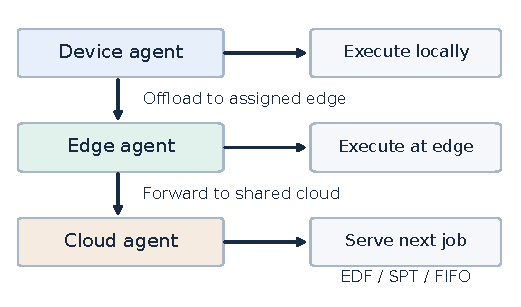
\includegraphics[width=\columnwidth]{figures/architecture.pdf}
\caption{Decision paths for the three agents. The device and edge can
execute at their own tier or escalate. The cloud chooses the service rule.}
\label{fig:architecture}
\end{figure}

\begin{figure}[t]
\centering
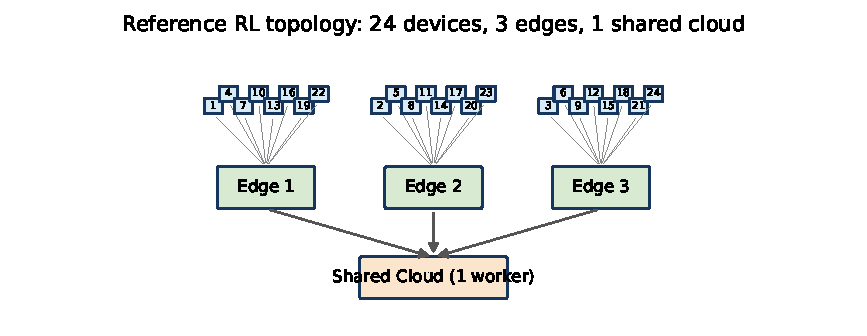
\includegraphics[width=\columnwidth]{figures/topology_24_devices.pdf}
\caption{Reference RL topology: 24 devices, three associated edges, and one
shared cloud worker.}
\label{fig:topology}
\end{figure}

\subsection{Task lifecycle and resource model}
The lifecycle is arrival, device decision, optional device--edge upload, edge
decision, optional edge--cloud upload, cloud dispatch, execution, and result
return. Queues contribute waiting time, and every modeled link contributes
serialization, propagation, and resource queue delay. Fig.~\ref{fig:lifecycle}
illustrates these paths.

\begin{figure}[t]
\centering
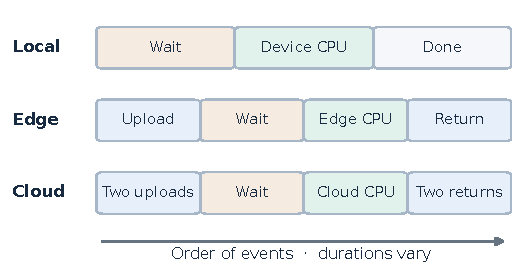
\includegraphics[width=\columnwidth]{figures/task_lifecycle.pdf}
\caption{Event order for the local, edge and cloud routes. Wait denotes
the compute queue. Transfers can also incur link queueing.}
\label{fig:lifecycle}
\end{figure}

Each task has arrival time, decimal-MB input and result sizes, required MI,
device identifier, relative deadline, and priority. For demand $w$ MI and
capacity $c$ MIPS,
\begin{equation}
t_{\mathrm{cpu}} = w/c.
\end{equation}
For payload $s$ decimal MB, bandwidth $B$ Mbps, propagation $p$, and queue
wait $q$,
\begin{equation}
t_{\mathrm{link}} = 8s/B+p+q.
\end{equation}
Latency is completion minus arrival, and a task meets its deadline when
$t_{\mathrm{completion}}\leq t_{\mathrm{arrival}}+D$. Devices and edges use
capacity-one SimPy resources. The current cloud has one worker and chooses
EDF, shortest processing time (SPT), or FIFO. Device energy includes CPU
energy per MI and transmit/receive power times radio duration; idle,
reception-infrastructure, retransmission, and cloud energy are not modeled.

\subsection{Observations and actions}
The device observation contains normalized work, input size, deadline slack,
battery fraction, device capacity, device--edge link state, and an optional
delayed edge-congestion signal. Its actions are local execution and edge
offloading. The edge observes task demand and deadline, edge queue/utilization,
edge capacity, edge--cloud link state, and an optional delayed cloud signal.
Its actions are edge execution and cloud forwarding. The cloud observes queue
length, deadline summaries, estimated service time, oldest wait, the count
of near-deadline jobs and workload imbalance. Device, edge and cloud use
11, 10 and 11 features. Work is log-scaled to compress its heavy tail.
The cloud chooses EDF (earliest absolute deadline), SPT (shortest
estimated service), or FIFO (first arrival to the cloud queue).
A centralized comparator uses a 16-feature
global observation and selects device, edge, or cloud, with fixed EDF cloud
dispatch. Lower-tier hierarchical agents do not receive raw global state.

\subsection{Learning and reward}
Q-learning estimates how much reward an agent can expect from an
action and the decisions that follow. For a policy $\pi$, the
action value is
\begin{equation}
Q^\pi(s,a)=
\mathbb E_\pi\!\left[\sum_{k=0}^{\infty}\gamma^k r_{t+k}
\mid s_t=s,\ a_t=a\right].
\end{equation}
Here $s$ is the observation used for control, $a$ is the action,
and $r_t$ is the reward assigned to the current decision. A
tabular Q-learning update adjusts the value of the observed pair
toward a target that combines the immediate reward and the best
estimated next action \cite{watkins1992}.
\begin{equation}
Q(s,a)\leftarrow Q(s,a)+
\alpha\left[r+\gamma\max_bQ(s',b)-Q(s,a)\right].
\end{equation}
The learning rate $\alpha$ controls the correction. At episode
termination the future term is zero.

Our observations include continuous quantities such as remaining
deadline, battery and queue wait. A table would require discretizing
their combinations. Deep Q-learning approximates $Q(s,a)$ with a
neural network. A Deep Q-Network (DQN) returns one score per
discrete action in a single pass. Fig.~\ref{fig:qnetwork} shows the
architecture used at each tier. The controller explores during
training and chooses the highest-scoring action during evaluation.

\begin{figure}[t]
\centering
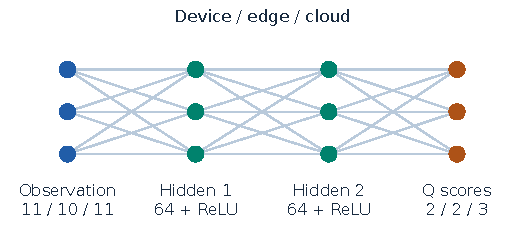
\includegraphics[width=\columnwidth]{figures/q_network.pdf}
\caption{DQN architecture shared by design across the three tiers.
Each controller has its own learned weights and input/output sizes.}
\label{fig:qnetwork}
\end{figure}

The DQN and Double DQN agents use two hidden layers of 64 units, replay
capacity 8,000, batch size 32, learning rate $3\mathord{\times}10^{-4}$,
target updates every 500 optimization steps, and Smooth L1 loss. Double DQN
selects the next action with the online network and evaluates it with the
target network. DQN takes the target-network maximum. Splitting selection
and evaluation addresses the upward bias that can arise when choosing
the largest of several noisy estimates \cite{hasselt2016double}.

For non-cloud decisions, the shared task reward is
\begin{equation}
\begin{aligned}
R=-\bigg(&w_l\min\left(1,\frac{\log(1+L/D)}{\log(10001)}\right)
+w_e\min\{3,E/E_0\}\\
&+w_d\mathbb{1}[\mathrm{miss}]
+w_c\min\{3,F/F_0\}\bigg),
\end{aligned}
\end{equation}
with $(w_l,w_e,w_d,w_c)=(0.35,0.25,0.35,0.05)$. Here $L$, $D$, $E$, and
$F$ denote end-to-end latency in seconds, deadline in seconds, device energy
in joules, and feedback bytes. The implementation uses $E_0=0.3$ J and
$F_0=64$ bytes from the default \texttt{RewardWeights} configuration; these
are normalization references, not measured campaign means. The miss indicator
is one when a deadline-feasible task misses its deadline. These weights
are design choices that trade off latency, device energy, feasible
deadline misses and feedback cost in a common scalar. The logarithm
compresses large latency ratios. In $\log(10001)$, the number 10,001
is $1+10{,}000$. At $L/D=10{,}000$, the normalized latency penalty
reaches one, and clipping caps it there. For example, with $L=2$ s,
$D=1$ s, $E=0.15$ J, $F=32$ B and a nominally feasible deadline, the
four weighted penalties are about 0.042, 0.125, 0.350 and 0.025.
The reward is their negative sum, approximately $-0.542$.
The cloud uses a
queue-waiting-cost reward for contested dispatches, so its objective is not
identical to the shared task reward.

The task reward is computed after completion and assigned to the decisions
on its route. The evaluated protocol links consecutive observations in each
controller's decision log, with $\gamma=0.9$ and a terminal transition
at the end of the log. Consecutive decisions can concern different tasks.
For reward $r$ and next observation $s'$, DQN uses
$y=r+\gamma\max_a Q_{\mathrm{target}}(s',a)$.
Double DQN selects $a^*=\arg\max_a Q_{\mathrm{online}}(s',a)$ and uses
$y=r+\gamma Q_{\mathrm{target}}(s',a^*)$. Both use $y=r$ at the final
transition.

The cloud reward is $-\min\{1,\log(1+n\hat t)/\log(10001)\}$,
where $n$ is the queue size at dispatch and $\hat t$ is the estimated
service duration in seconds. This proxy for queue occupancy during
service favors shorter jobs at a given queue size. Singleton queues are
omitted from cloud replay because the three rules select the same job.
\subsection{Feedback}
Feedback is adjacent-tier and causal. A snapshot sampled at time $t$ is
available only after modeled propagation and serialization, at a later
decision. Conditions are none, periodic, frequent, and event-triggered. The
event trigger sends an initial snapshot, sends when the signal change reaches a
threshold, and refreshes after five observations. Feedback bytes, modeled
delay, and information age are recorded. At a decision, information age is
the elapsed time since the consumed snapshot was sampled \cite{yatesAoI}.
The modeled control path operates independently of data-plane queues. Fig.~\ref{fig:coordination} shows this control path.

\begin{figure}[t]
\centering
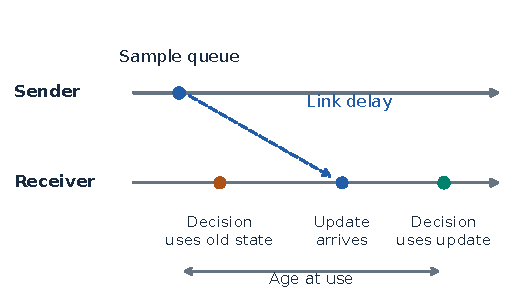
\includegraphics[width=\columnwidth]{figures/coordination.pdf}
\caption{Timing of a queue snapshot sent to the neighboring tier.
Information age is measured from sampling to the decision that uses it.}
\label{fig:coordination}
\end{figure}

\section{Proposed Hierarchical Method}
\subsection{Policy contracts}
The device observes normalized task demand, input size, deadline slack,
battery fraction, local capacity, and device--edge link information, with an
optional delayed edge-congestion signal. Its actions are local execution and
edge offloading. The edge observes queue/utilization, task demand and
deadline, edge--cloud link state, and an optional delayed cloud signal. Its
actions are edge execution and cloud forwarding. The cloud observes queue
length, deadline summaries, estimated execution time, and wait time; its
actions are EDF, shortest processing time, and FIFO. The centralized comparator
uses a 15-feature observation and selects device, edge, or cloud; cloud
dispatch remains EDF.

\subsection{Reward and learning formulation}
For a task result $r$, the implemented team reward is
\begin{equation}
R=-\left(w_l\min(3,L/D)+w_e\min(3,E/E_0)
w_d\mathbb{1}[\mathrm{miss}]
w_c\min(3,F/F_0)\right),
\end{equation}
where $L$ is latency, $D$ the task deadline, $E$ device energy, $F$ feedback
bytes, and $(E_0,F_0)$ normalization references. The default weights are
$(0.35,0.25,0.35,0.05)$.

Each decision is stored with its own task identifier. Credit is assigned only
after that task's terminal result is available, with a zero next observation
and \texttt{done=True}. This is a contextual one-step learning formulation
implemented with a Double-DQN replay learner, not a sequential multi-step
MDP. Fig.~\ref{fig:rl} summarizes this distinction.

\begin{figure}[t]
\centering
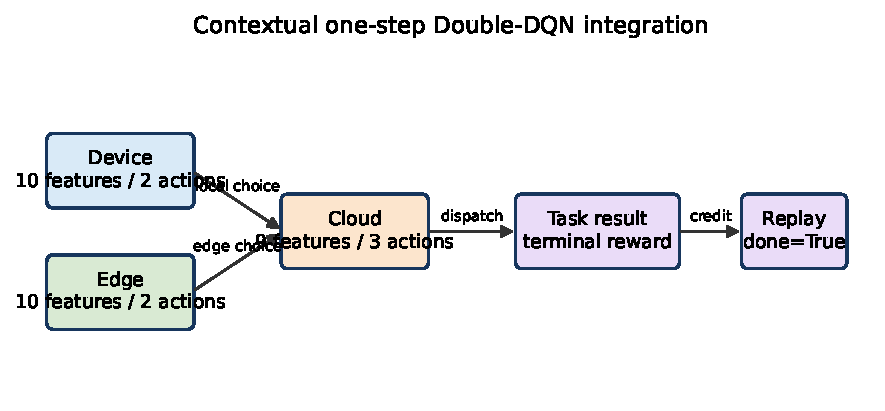
\includegraphics[width=\columnwidth]{figures/hierarchical_rl.pdf}
\caption{Local observations and terminal per-task credit.}
\label{fig:rl}
\end{figure}

\subsection{Coordination}
Feedback is adjacent-tier and causal: a message sampled at time $t$ becomes
available after propagation plus serialization at a later decision. Modes are
none, periodic, and frequent. Messages contribute recorded bytes and modeled
delay, but they do not contend with data-plane resources or block execution.
Thus the implementation measures control-plane accounting, not a complete
communication-latency trade-off. Fig.~\ref{fig:coordination} shows the
implemented information path.

\begin{figure}[t]
\centering
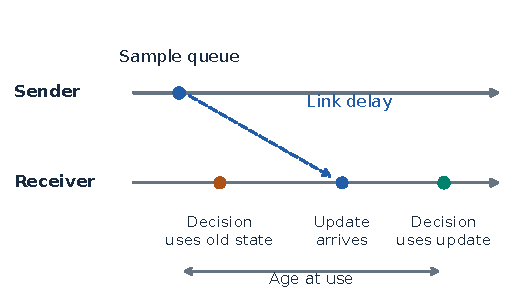
\includegraphics[width=\columnwidth]{figures/coordination.pdf}
\caption{Delayed adjacent-tier feedback; control traffic is non-blocking.}
\label{fig:coordination}
\end{figure}

\section{Implementation and Performance Evaluation}
\subsection{Software and reproducibility}
The implementation targets Python 3.11 and uses SimPy for event scheduling, PyTorch for learning, and
NumPy, pandas, Matplotlib and PyYAML for workload preparation and analysis.
For the six-policy comparison, we matched task identifiers and arrival
timestamps, verified the trace and topology fingerprints, and checked
that training, validation and evaluation noise seeds were disjoint.
The resulting dataset contains 52,110 task outcomes and 90 replay
summaries. A 20-task pilot with each algorithm verified that all
policies ran on the same reference configuration.

\subsection{Dataset and workload construction}
Alibaba Cluster Trace 2017 records a 24-hour period from part of a
production cluster that runs batch jobs and online services
\cite{alibaba2017}. We use the batch task and instance tables. The task
table supplies creation time and the job and task identifiers. The
instance table supplies start and finish timestamps and average CPU
use in cores. We join the two tables by job and task identifiers.

We retain completed tasks belonging to single-task jobs with at least
one valid completed instance. For task $i$, the work in million
instructions (MI) is derived as
\begin{equation}
w_i=\frac{c_{\rm ref}}{|\mathcal I_i|}
\sum_{j\in\mathcal I_i}(t^{\rm end}_j-t^{\rm start}_j)u_j,
\end{equation}
where $\mathcal I_i$ contains valid completed instances, $u_j$ is
average CPU use and $c_{\rm ref}=1000$ MIPS per core is a modeling
constant. The average represents a typical instance. Summing across
parallel instances would map their combined work onto one sequential
service. The filter retains 2,891 of 80,553 task records. In the
separate instance table, 147,849 records are flagged for malformed
fields or invalid completed-instance measurements.

The accepted tasks are sorted by arrival and split chronologically
into 1,734 training, 578 validation and 579 test tasks.
Fig.~\ref{fig:workload} shows the compute-demand quantiles by split.

\begin{figure}[t]
\centering
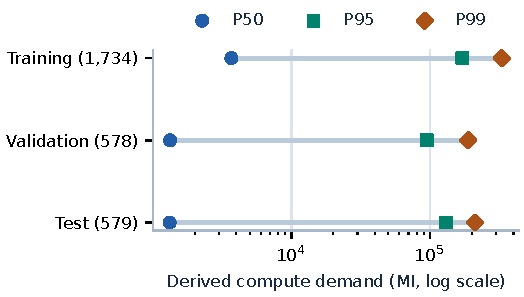
\includegraphics[width=\columnwidth]{figures/workload_quantiles.pdf}
\caption{Compute demand after trace adaptation. Each row reports
the median, P95 and P99 for one chronological split.}
\label{fig:workload}
\end{figure}

The accepted test tasks span 9,753 trace seconds. Their median work is
1,320 MI and their P95 work is 131,057 MI. The six largest tasks account
for 14.5\% of the test workload. A P95-sized task takes about 6.55 s
of nominal service even at 20,000 MIPS. A single worker can therefore
remain occupied while several smaller jobs arrive.

The evaluation uses the best-tier-calibrated deadline rule with a one-second
floor and validation-calibrated arrival compression
$0.12793575549650835$. Payload sizes, device assignment, device battery and
radio state, wireless bandwidth and propagation, edge/cloud capacities, and
relative deadlines are simulator assumptions. Input size is assigned
reproducibly per task using a lognormal distribution with median 1 MB,
log-scale standard deviation 1 and a cap of 50 MB. The result returned
to the device is 0.1 MB. Tasks are assigned round-robin to 24 devices
with fixed edge associations. The test median interarrival time changes
from 10 s in the trace to 1.28 s after compression. The dataset
therefore supplies workload timing and compute demand, while the
simulator defines the mobile network and deadline regime.

\subsection{Matched evaluation protocol}

The primary comparison uses 579 tasks on the reference topology: 24 devices,
three edges, and one cloud worker. Random, Greedy/FIFO, and Greedy/EDF are
fixed baselines evaluated with noise seeds 10001--10005. Centralized DQN uses
the five standard-DQN checkpoints from training seeds 42--46, observes global
state, and uses fixed EDF cloud dispatch. Hierarchical DQN and hierarchical
Double DQN use the ten frequent-feedback bundles at the same five training
seeds; their cloud rules are learned. For learned policies, five noise runs
are averaged within each training seed, then the mean and sample standard
deviation are computed across five training-seed means. Baseline deviations
are across the five noise seeds. P95 is computed per replay before
aggregation, so these two SDs describe different variation sources.

\begin{table}[t]
\centering
\caption{Reference simulation and training settings.}
\label{tab:settings}
\small
\begin{tabular}{@{}p{.31\columnwidth}p{.63\columnwidth}@{}}
\toprule
Parameter & Setting \\
\midrule
Compute capacity & Device 800/1,000/1,200 MIPS, edge
5,000/6,250/7,500 MIPS, cloud 20,000 MIPS \\
Device--edge link & 100 Mb/s, 10 ms propagation \\
Edge--cloud link & 1,000 Mb/s, 40 ms propagation \\
Timing noise & Bandwidth and service perturbations of up to 10\% \\
Relative deadline & $\max\{1,\,0.9w/20000+0.5\}$ s, with $w$ in MI \\
Training & Up to 1,000 episodes of 100 tasks, nine training topologies \\
Exploration & Linear from 0.90 to 0.05 over the first 75\% of the budget \\
Validation & 578 tasks, five noise seeds, every 25 episodes \\
\bottomrule
\end{tabular}
\end{table}

Table~\ref{tab:settings} lists the main settings. Checkpoint selection
maximizes validation deadline success and uses lower P95 to break ties.
Training stops early after eight validation checks without improvement
for both learners. For the test, the original deadline
formula stays fixed when changing topology.

\subsection{Matched six-policy comparison}
Table~\ref{tab:matched} is the primary result. Device energy is reported in
joules per task. Reported means and standard deviations summarize the
observed replays.

\begin{table}[t]
\centering
\caption{Matched reference-topology comparison. Means $\pm$ SD; P95 is per
replay before aggregation.}
\label{tab:matched}
\scriptsize
\resizebox{\columnwidth}{!}{%
\begin{tabular}{lrrr}
\toprule
Policy & Deadline success (\%) & P95 latency (s) & Device energy (J/task)\\
\midrule
Random & $49.57\pm0.95$ & $137.96\pm16.46$ & $10.480\pm0.720$\\
Greedy/FIFO & $75.79\pm0.78$ & $13.62\pm0.49$ & $0.211\pm0.001$\\
Greedy/EDF & $75.89\pm0.86$ & $12.95\pm0.43$ & $0.211\pm0.001$\\
Centralized DQN & $77.41\pm1.37$ & $15.71\pm4.44$ & $0.242\pm0.067$\\
Hierarchical DQN & $74.63\pm0.79$ & $16.91\pm3.32$ & $0.260\pm0.104$\\
Hierarchical Double DQN & $74.33\pm1.66$ & $15.08\pm2.85$ & $0.244\pm0.065$\\
\bottomrule
\end{tabular}}
\end{table}

\begin{table}[t]
\centering
\caption{Mean latency and communication. Means $\pm$ SD. Data and feedback
volumes are per 579-task replay.}
\label{tab:matched-extra}
\tiny
\setlength{\tabcolsep}{2pt}
\begin{tabular}{@{}lrrr@{}}
\toprule
Policy & Mean $L$ (s) & Data ($10^8$ B) & Feedback ($10^3$ B)\\
\midrule
Random & $22.002\pm2.681$ & $8.07\pm0.57$ & $0$\\
G/FIFO & $2.619\pm0.046$ & $12.86\pm0.12$ & $0$\\
G/EDF & $2.472\pm0.088$ & $12.86\pm0.12$ & $0$\\
C-DQN & $2.794\pm0.447$ & $12.54\pm0.68$ & $0$\\
H-DQN & $3.045\pm0.292$ & $12.72\pm1.08$ & $35.4\pm0.7$\\
H-DDQN & $3.015\pm0.470$ & $12.04\pm0.42$ & $35.1\pm0.6$\\
\bottomrule
\end{tabular}
\end{table}

Figure~\ref{fig:matched} visualizes the same documented summary. Centralized
DQN has the highest mean success, while Greedy/EDF has the lowest mean P95.
Greedy/FIFO and Greedy/EDF share the lowest mean energy. Both hierarchical
learners improve on Random across all three headline metrics, while the
reference comparison exposes different strengths for centralized control,
heuristic scheduling, and hierarchy. Double DQN lowers mean P95 and energy
relative to hierarchical DQN, with a small success decrease. These are
descriptive comparisons, not claims of statistical significance.

\begin{figure*}[t]
\centering
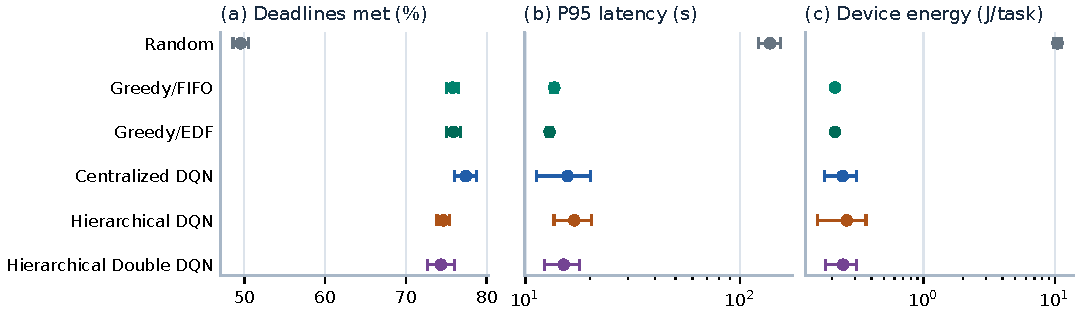
\includegraphics[width=\textwidth]{figures/final_matched_comparison.pdf}
\caption{Matched-policy comparison. Points are means and whiskers are
one sample standard deviation across training-seed means for learned
policies or across noise seeds for fixed policies. Latency and energy
use logarithmic axes.}
\label{fig:matched}
\end{figure*}

\begin{figure}[t]
\centering
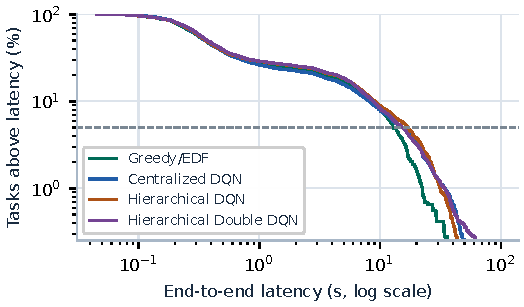
\includegraphics[width=\columnwidth]{figures/latency_tail.pdf}
\caption{Empirical latency exceedance for four policies. The dashed line
marks 5\%. The curves pool the same held-out tasks over the available
replays per policy. Table~\ref{tab:matched} averages per-replay P95 values.}
\label{fig:latency-tail}
\end{figure}

Fig.~\ref{fig:latency-tail} shows why the P95 matters. Hierarchical
DQN has a mean latency of 3.04 s and a mean per-replay P95 of
16.91 s. The high tail includes queuing, execution and transfers.
It indicates a risk for latency-sensitive IoT applications under
this compute-heavy workload and modeled contention.

\paragraph{Additional centralized control}
The primary table uses one centralized reference. As an additional
control, we evaluated the five centralized Double DQN checkpoints
under the same trace, reference topology, and five noise seeds. This
variant uses fixed EDF in the cloud and obtains $77.40\pm1.24$\%
deadline success, $13.74\pm2.08$ s P95, and $0.224\pm0.026$ J/task.
The two centralized variants have nearly identical mean success.
Centralized Double DQN has a lower mean P95, while Greedy/EDF
retains the lowest mean P95 of the evaluated policies. The
centralized control separates the choice of learning target from
the choice of information and control architecture, although
centralized and hierarchical cloud dispatch differ.

\subsection{Feedback and topology sensitivity}
To isolate feedback settings, each algorithm was evaluated with five
training seeds under each condition. Table~\ref{tab:feedback} compares
frequent updates with event-triggered updates at the checkpoint's
trained threshold. Traffic is measured per 579-task replay.

\begin{table}[t]
\centering
\caption{Coordination trade-off on the reference topology.}
\label{tab:feedback}
\footnotesize
\setlength{\tabcolsep}{4pt}
\begin{tabular}{@{}llrrr@{}}
\toprule
Learner & Mode & Success (\%) & P95 (s) & Feedback (kB) \\
\midrule
DQN & Frequent & 74.63 & 16.91 & 35.39 \\
DQN & Event 0.10 & 75.74 & 18.84 & 11.86 \\
DQN & Event 0.25 & 73.07 & 16.61 & 11.99 \\
DQN & Event 0.50 & 74.75 & 16.74 & 10.69 \\
Double DQN & Frequent & 74.33 & 15.08 & 35.13 \\
Double DQN & Event 0.10 & 74.29 & 17.00 & 11.53 \\
Double DQN & Event 0.25 & 74.95 & 17.46 & 11.09 \\
Double DQN & Event 0.50 & 74.98 & 17.80 & 10.43 \\
\bottomrule
\end{tabular}
\end{table}

At threshold 0.50, Double DQN reduces feedback traffic by 70.3\%
relative to frequent feedback, with a 0.65 percentage point increase
in observed success and a 2.72 s increase in P95. For DQN, the same
comparison reduces feedback bytes by 69.8\%, with a 0.12 point
increase in observed success and a 0.17 s decrease in P95.
These comparisons use separately trained policies and the cost
includes feedback bytes. They describe the combined effect of the
feedback mechanism and learning under that mechanism.

Four variants probe transfer to resource settings held out during
training. They increase cloud CPU, improve the device--edge link,
improve the edge--cloud link, or combine reduced CPU and link
capacity with longer propagation. Under combined stress and
frequent feedback, DQN reaches 61.73\% success and 29.42 s P95,
compared with 60.17\% and 40.41 s for Double DQN. The reference
latency ranking reverses in this condition. The matched evaluation
therefore supports conclusions tied to a workload and topology.

\subsection{Cloud scheduling with frozen upstream policies}
The cloud ablation replays each frequent-feedback checkpoint with
the learned rule selector and each fixed rule, keeping device and
edge weights, tasks and noise seeds paired. The results in
Table~\ref{tab:cloud} show the effect of switching the cloud scheduler
under the same upstream policies.

\begin{table}[t]
\centering
\caption{Cloud ablation on the reference topology.}
\label{tab:cloud}
\footnotesize
\begin{tabular}{@{}lrrrr@{}}
\toprule
 & \multicolumn{2}{c}{DQN upstream} & \multicolumn{2}{c}{Double DQN upstream} \\
Rule & Success (\%) & P95 (s) & Success (\%) & P95 (s) \\
\midrule
Learned & 74.63 & 16.91 & 74.33 & 15.08 \\
EDF & 74.65 & 16.37 & 74.24 & 15.29 \\
SPT & 75.23 & 12.26 & 74.82 & 12.36 \\
FIFO & 74.25 & 18.25 & 73.90 & 17.82 \\
\bottomrule
\end{tabular}
\end{table}

SPT gives the highest mean success and lowest mean P95 for both
upstream architectures across the five tested topologies. With the
Double DQN upstream policy on the reference, SPT reduces P95 by
2.72 s relative to its learned scheduler. All ten checkpoints
consistently select one rule whenever multiple jobs are queued, and
the corresponding fixed-rule replay reproduces their per-task
outcomes. This explains why evaluating against all three fixed rules
matters. An improvement over EDF alone could reflect the choice of a
different fixed rule. The long tail of task work and the short-service
preference in the cloud reward help explain the competitive SPT result.

\subsection{Reporting limitations}
The evaluation reports mean latency, P95 latency, deadline success,
device energy, task communication bytes, and feedback bytes; Table~\ref{tab:matched-extra}
adds the metrics not included in Table~\ref{tab:matched}. Device energy is
total modeled device CPU
and radio energy divided by the tasks in a replay, then aggregated according
to the seed aggregation described above. It excludes idle,
reception-infrastructure, retransmission, and cloud energy. Task communication bytes are data-plane payload bytes; feedback bytes are
control-plane bytes. Feedback currently does not contend with data-plane
links, so its communication cost should not be interpreted as queueing
interference.

Centralized DQN observes global state and therefore has an information
advantage over the hierarchical policies; centralized state-collection
traffic is not included in the communication accounting. The five evaluation
seeds vary simulated bandwidth and service-time noise on one chronological
test window, not five independent trace periods, and the five training seeds
provide limited evidence. The reported standard deviations are descriptive
and reflect different aggregation sources for fixed and learned policies.

\section{Performance Evaluation}
\subsection{Evidence audit}
Table~\ref{tab:evidence} distinguishes source implementation, tests, and
committed experimental evidence. This distinction is essential because a
policy constructor or test does not establish a performance improvement.

\begin{table}[t]
\centering
\caption{Evidence status at the audited repository revision.}
\label{tab:evidence}
\scriptsize
\resizebox{\columnwidth}{!}{%
\begin{tabular}{p{.31\columnwidth}p{.18\columnwidth}p{.39\columnwidth}}
\toprule
Capability & Status & Evidence boundary\\
\midrule
Multi-device topology & implemented/tested & explicit topology code and tests; no final campaign\\
Multi-edge/shared cloud & implemented/tested & backend and topology configuration; no final campaign\\
Random, greedy, EDF & implemented/validated & committed three-seed synthetic CSV; controlled scenario tests\\
Device/edge/cloud RL & implemented/tested & adapters, observations, credit tests; no committed run\\
Centralized RL & implemented/tested & centralized adapter and tests; no committed run\\
Hierarchical coordination & implemented/tested & causal feedback unit tests; no final ablation\\
Alibaba workload & adapter/tested & mapping and loader tests; no committed trace results\\
Feedback overhead & modeled/tested & counters and theoretical delay; non-blocking\\
\bottomrule
\end{tabular}
}
\end{table}

\subsection{Committed baseline results}
The same seeded workload is passed to every policy. Table~\ref{tab:baselines}
reports the mean across three seeds and the sample standard deviation from
\texttt{results/dev-smoke/aggregate\_statistics.csv}.

\begin{table}[t]
\centering
\caption{Three-seed synthetic baseline evidence (mean $\pm$ standard deviation).}
\label{tab:baselines}
\scriptsize
\resizebox{\columnwidth}{!}{%
\begin{tabular}{lrrrr}
\toprule
Policy & Mean L (s) & P95 L (s) & Deadline & Energy (J)\\
\midrule
Local & 3.164 $\pm$ .467 & 5.491 $\pm$ .612 & 36.7\% & .619 $\pm$ .072\\
Greedy/edge & .602 $\pm$ .118 & .927 $\pm$ .137 & 100\% & .565 $\pm$ .165\\
Edge execute & .602 $\pm$ .118 & .927 $\pm$ .137 & 100\% & .565 $\pm$ .165\\
Cloud/EDF & .513 $\pm$ .113 & .745 $\pm$ .160 & 100\% & .565 $\pm$ .165\\
Cloud/FIFO & .513 $\pm$ .113 & .745 $\pm$ .160 & 100\% & .565 $\pm$ .165\\
Random & 1.177 $\pm$ .387 & 2.625 $\pm$ .761 & 90.0\% & .424 $\pm$ .067\\
\bottomrule
\end{tabular}
}
\end{table}

Cloud forwarding has the lowest mean latency in this light synthetic
workload, but it doubles the modeled payload traffic relative to edge
execution (27.48 MB versus 13.74 MB per seed-average aggregate). Local
execution consumes more device CPU energy and misses more deadlines. These
observations are scenario-specific: greedy/edge equals edge execution because
all default tasks satisfy the greedy offload inequality, and EDF equals FIFO
because the smoke workload does not create a meaningful cloud ordering choice.
The controlled contention scenario distinguishes their queue order but still
misses its deliberately urgent task under both policies.

\subsection{Unvalidated comparisons}
The repository contains scripts for centralized RL, hierarchical RL, three
feedback modes, and synthetic load/network scenarios. It does not contain the
models, comparison CSVs, or run logs needed to reproduce those measurements at
the audited revision. Accordingly, no RL ranking, convergence, topology
sensitivity, feedback benefit, or Alibaba improvement is reported. The
required next experiment is to run training and held-out evaluation with
disjoint seeds, then export the configured metrics and metadata alongside the
commit and package versions.

\section{Conclusion and Perspectives}
The three-tier framework makes placement, cloud scheduling and coordination
measurable under paired task replays. On the reference topology,
centralized DQN reaches 77.41\% deadline success, and the additional
centralized Double DQN control reaches 77.40\%. Greedy/EDF achieves
the lowest mean P95, at 12.95 s. Among hierarchical controllers,
Double DQN reduces the reference P95 from 16.91 to 15.08 s relative
to DQN, with a 0.30 percentage point decrease in deadline success.
The latency ranking reverses under combined stress.

The frozen-policy ablation identifies SPT as the strongest cloud rule
on the tested workloads. On the reference, replacing the learned
Double DQN cloud scheduler by SPT reduces mean P95 from 15.08 to
12.36 s with the same upstream weights. The event-triggered feedback
experiment also identifies a practical control mechanism. At
threshold 0.50, Double DQN transmits about 70\% fewer feedback bytes
than with frequent updates, with a 2.72 s increase in mean P95.

These results characterize one chronological test window and a
single-worker cloud. An independent trace period, multi-worker
execution and a shared data/control network would extend the
evaluation. Federated training is a further direction. Devices could
aggregate local updates at each edge before the edges synchronize at
the cloud, with synchronization traffic measured separately from
inference feedback.


\bibliographystyle{IEEEtran}
\bibliography{references}
\end{document}
